\section{Optimal Control of Pitch/Travel without Feedback}\label{sec:prob2}

In this section we will calculate an optimal trajectory $x^*$ and a
corresponding optimal input sequence $u^*$, that will bring the helicopter
from a given initial state to a desired final state. The computation of the
optimal trajectory is formulated as a discrete convex optimization problem.

\subsection{State-space formulation}
The system (\ref{eq:model_al}) describes the helicopter plant, with a basic
PID controller for the elevation and a PD controller for the pitch. In this
section we will disregard elevation, that is, we assume $e = 0$. The system
can then be written on the continuous-time state-space form,
\begin{equation}
    \dot{x} = A_cx + B_cu
    \label{eq:state_space_axbu}
\end{equation}
with $x = \begin{bmatrix} \lambda & r & p & \dot{p} \end{bmatrix}^T$ and $u = p_c$.
The corresponding continuous-time system matrices are
\begin{equation}
	A_c = \begin{bmatrix} 0 & 1 & 0 & 0 \\ 0 & 0 & -K_2 & 0 \\ 0 & 0 & 0 & 1 \\ 0 & 0 & -K_1K_{pp} & -K_1K_{pd} \end{bmatrix}
	\qquad\text{and}\qquad
	B_c = \begin{bmatrix}0 \\ 0 \\ 0 \\K_1K_{pp} \end{bmatrix}
\end{equation}
Referring to the control hierarchy layer in figure (\ref{fig:control_hierarchy}),
this is a model of the basic control layer and the physical layer. In this section
we will implement part of the optimization layer.
\begin{figure}[ht]
	\centering
	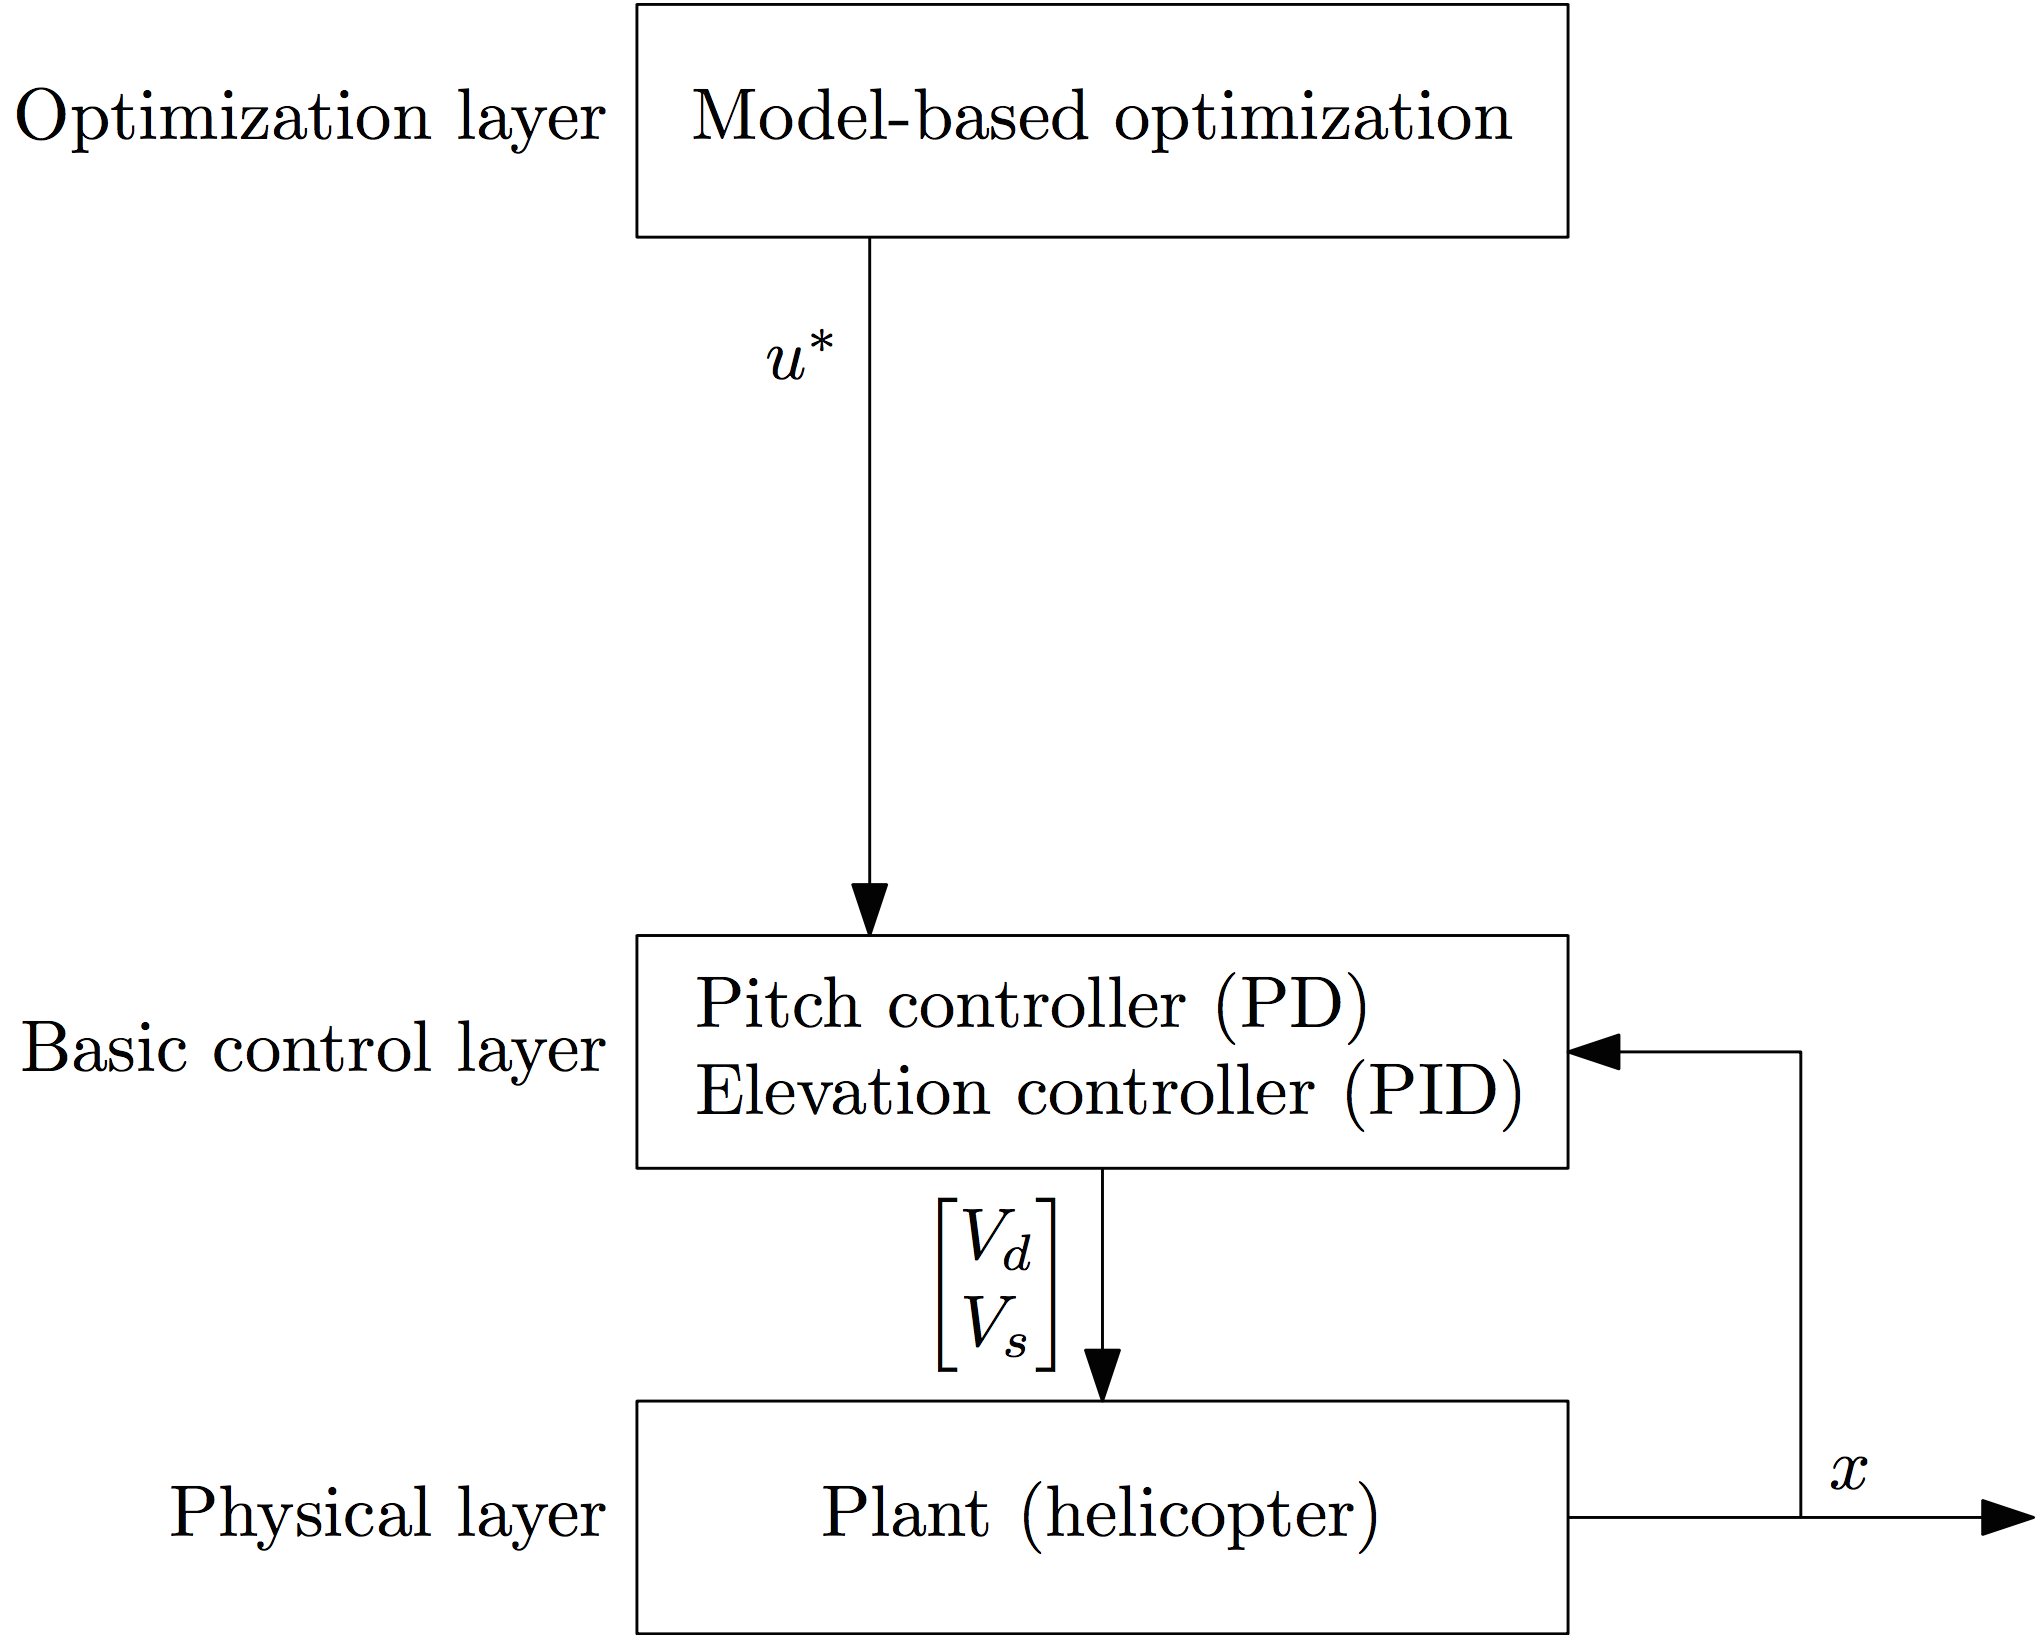
\includegraphics[width=0.6\textwidth]{figures/control_hierarchy_day2}
	\caption{Control hierarchy}
	\label{fig:control_hierarchy}
\end{figure}

\subsection{Discretization}
The system dynamics will be implemented as a sequence of constraints in the
optimization problem, and must therefore be written in discrete-time state-
space form,
\begin{equation}
	x_{k+1} = Ax_k + Bu_k
	\label{eq:discrete_state_space_axbu}
\end{equation}
We discretize the model using forward-Euler by approximating derivatives
with a forward difference over the timestep $h$,
\begin{equation}
	\dot{x}_k \approx \frac{x_{k+1} - x_k}{h}
\end{equation}
Inserting this into (\ref{eq:state_space_axbu}) we find
\begin{equation}
	\dot{x}_{k+1} \approx (I + hA_c) x_k + hB_c u_k
\end{equation}
A suitable approximation for the discrete-time matrices is then
\begin{equation}
	A \approx I + hA_c
	\qquad\text{and}\qquad
	B \approx hB_c
\end{equation}


\subsection{Computation of optimal trajectory}
An optimal trajectory can be generated by minimizing the cost function
\begin{equation}
	\label{eq:trajectory_cost}
	\phi = \sum_{i=1}^{N}(\lambda_i - \lambda_f)^2 + qp_{ci}^2
\end{equation}
for some scalar weight $q \geq 0$ over the finite horizon of states and inputs
\begin{equation}
	z = (x_1 \; x_2 \; ... \; x_N \; u_1 \; u_2 \; ... \; u_N)^T
\end{equation}
The discrete-time system dynamics are implemented as equality constraints of the form $A_{\text{eq}}z = B_{\text{eq}}$, where $A_{\text{eq}}$ and $B_{\text{eq}}$ are given by the left- and right-hand side of the $N$ constraints
\begin{align*}
	x_1 - Bu_0        &= Ax_0 \\
	x_2 - Ax_1 - Bu_1 &= 0    \\
	\vdots                    \\
	x_N - Ax_{N-1} - Bu_{N-1} &= 0
\end{align*}
We would also like to constrain the system state and input to be within a range
\begin{align}
	x^{\text{min}} \leq x_{t+1} \leq x^{\text{max}} \\
	u^{\text{min}} \leq u_t \leq u^{\text{max}}
\end{align}
for $t = 0...N-1$. Applying these constraints to all states and inputs in the solution horizon, we have
\begin{equation}
	\begin{bmatrix} I \\ -I \end{bmatrix} z
	\leq
	\begin{bmatrix}
	\{x_{t+1}^{max}\} \\
	\{u_t^{max}\} \\
	\{x_{t+1}^{min}\} \\
	\{u_t^{min}\}
	\end{bmatrix}_{t=0..N-1}
\end{equation}
which can be implemented as an inequality constraint of the form $A_{\text{iq}} z \leq B_{\text{iq}}$.

Note that the cost function (\ref{eq:trajectory_cost}) does not take into consideration that $\lambda_i$ plus some multiple of $2\pi$ describes the same physical orientation of the helicopter. For example, if the reference is $0$ and $\lambda_i = 2\pi$, it will be regarded as a large error, even though the helicopter is infact in the desired orientation. A more optimal scheme would take this into consideration.

\subsection{Results}

% TODO: Add figure showing that the helicopter does NOT end up in our desired final state, xf.
\begin{figure}[htb]
	\centering
    	\makebox[\textwidth][c]{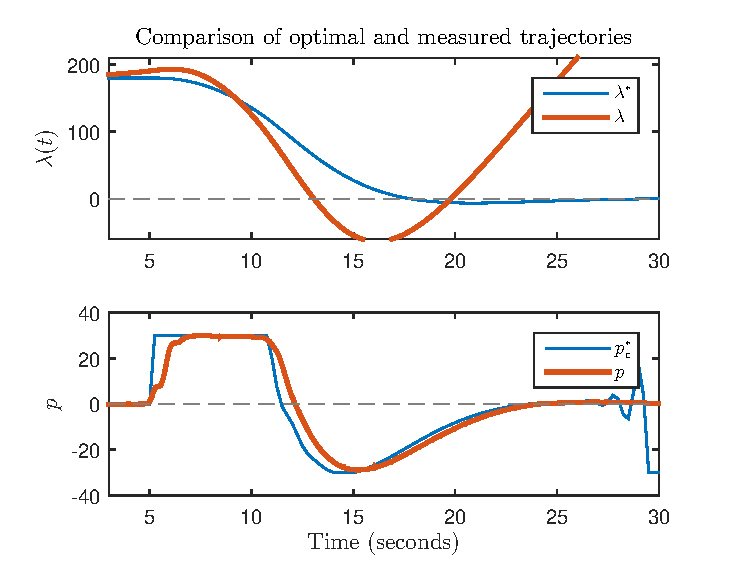
\includegraphics[width=\textwidth]{figures/day2/plot_day2}}
	\caption{Plot of day 2}
	\label{fig:day2_plot}
\end{figure}

% TODO: Explain WHY the helicopter does not reach the final state. Why was the computed trajectory not optimal in the physical sense? etc...

% Grunner til at den beregnede optimale banen gir ugunstig resultat:
%     * I modellen antar vi at pitch-regulatoren er såpass kjapp, at pitch vil være nøyaktig like pitch-referanse til enhver tid. Dette er åpenbart feil. Men den største grunnen er:

%     * Diverse andre modelleringsfeil gjør at den beregnede pådragssekvensen ikke er den fysisk optimale sekvensen. Hadde modellen vært perfekt, ville helikopteret fulgt banen. Feedback kan hjelpe med å kjempe mot modelleringsfeil.
